%------------------------------------------------------------------------------------------------------------
\section{Data structures} \label{sec:DataStructures}
%------------------------------------------------------------------------------------------------------------

An overview of the data structures implemented in the AMIDST toolbox is illustrated in Figure \ref{Figure:ToolboxDataStructures}. These data structures basically define the main components that will be used afterwards for implementing the AMIDST learning and inference algorithms. As we previously mentioned, in the AMIDST toolbox, we focus on two specific instantiations of PGMs, namely, a static Bayesian network (\comp{BN} component) and a two time-slice dynamic Bayesian network (\comp{2T-DBN} component). 

\vspace{-0.1in}

\begin{figure}[ht!]
\begin{center}
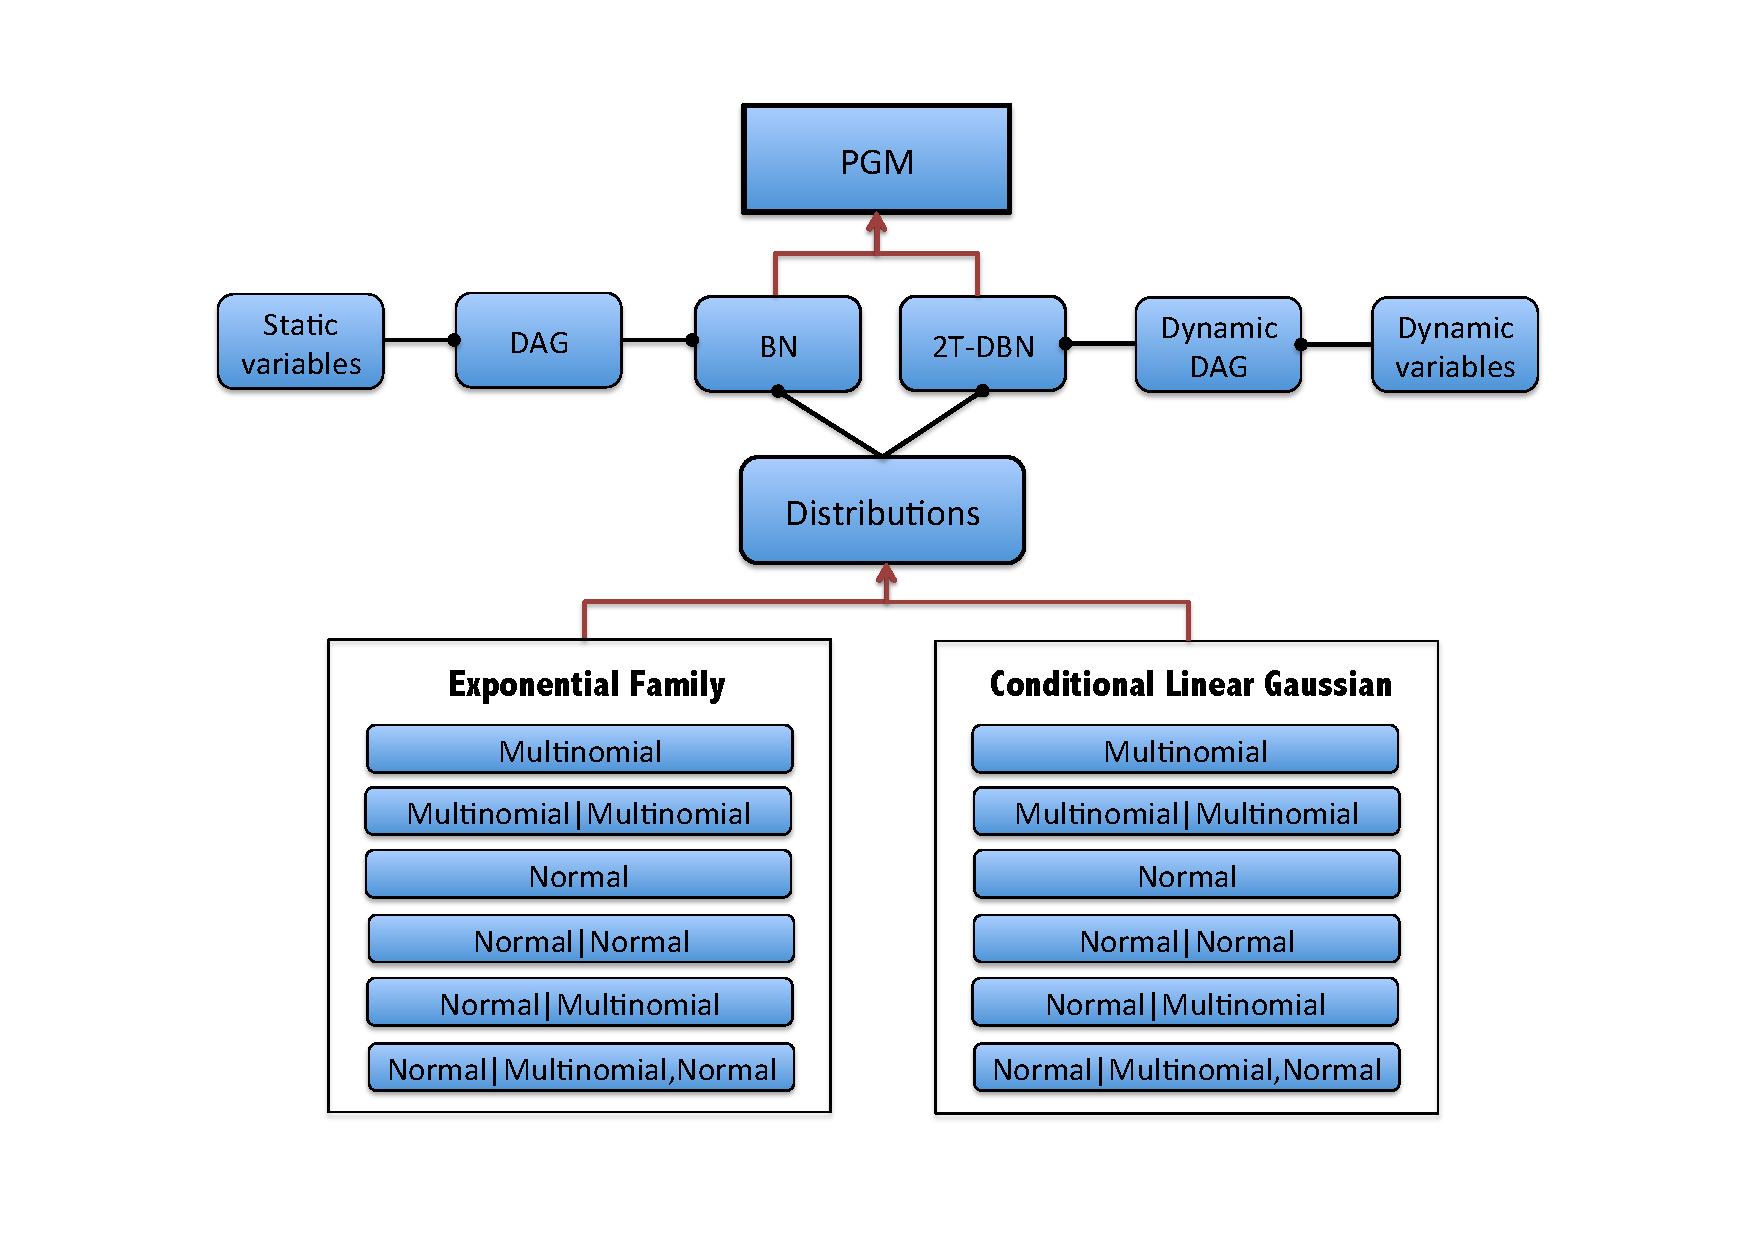
\includegraphics[width=\linewidth]{./figures/DataStructure}
\vspace{-0.5in}
\caption{\label{Figure:ToolboxDataStructures} Illustration of AMIDST toolbox data structure components. Nomenclature: The boxes in the
      figure represent software components (sets, possibly singletons, of classes), a rounded-arc going from $X$ to $Y$ indicates that $Y$ 'uses/references' $X$, and an arc with an arrow from $X$ to $Y$ implies inheritance.}
\end{center}
\end{figure}

In what follows, we briefly define each component and how it can be used in AMIDST toolbox through providing some code excerpts.  

%------------------------------------------------------------------------------------------------------------
\subsection{Static variables}
%------------------------------------------------------------------------------------------------------------

Static variables consist of a list of objects of type Variable that are used later to build a static BN. Each static variable is characterized by its name, ID, the state space type, the distribution type (i.e., multinomial or normal), as well as if it is observed or not. 

Note that observed static variables are initialised using the list of attributes (that are already parsed from the dataset or specified by the user), then hidden static variables could be afterwards specified by the user.

The following source code example shows how to define a set of four static observable variables and a single hidden variable:

\vspace{-0.1in}
\begin{table}[H]
\begin{tabular}{l} \\ \hline

        \texttt{DataStream<DataInstance> data = }\\
        
        \texttt{~~~~~~~~~~DataStreamLoader.loadFromFile("datasets/staticData.arff");}\\

        \texttt{StaticVariables variables = new StaticVariables(data.getAttributes());}\\

        \texttt{Variable A = variables.getVariableByName("A");}\\
        \texttt{Variable B = variables.getVariableByName("B");}\\
        \texttt{Variable C = variables.getVariableByName("C");}\\
        \texttt{Variable D = variables.getVariableByName("D");}\\

        \texttt{Variable H = variables.newMultionomialVariable("HiddenVar",}\\ \texttt{~~~~~~~~~~~~~~~~~~~~~~~~~Arrays.asList("TRUE", "FALSE"));}\\ \hline 

\end{tabular}
\end{table}


%------------------------------------------------------------------------------------------------------------
\subsection{Directed acyclic graph (\comp{DAG})}
%------------------------------------------------------------------------------------------------------------

A directed acyclic graph (\comp{DAG}) defines the BN graphical structure over a list of \comp{static variables}, such that the dependence relationships between the variables are established through the definition of the parent set for each variable. 

The following source code example shows how to build a \comp{DAG} over the previously defined set of static variables, such that the hidden variable is set as a parent of all the remaining variables:

\vspace{-0.1in}
\begin{table}[H]
\begin{tabular}{l} \\ \hline

        \texttt{DAG dag = new DAG(variables);}\\\\

        \texttt{dag.getParentSet(A).addParent(H);}\\
        \texttt{dag.getParentSet(B).addParent(H);}\\
        \texttt{dag.getParentSet(C).addParent(H);}\\
        \texttt{dag.getParentSet(D).addParent(H);}\\\\
        
        \texttt{System.out.println(dag.toString());}\\\hline 

\end{tabular}
\end{table}

The last line converts the resulting \texttt{dag} into a String object, then prints it to the standard console. We obtain:

\vspace{-0.1in}
\begin{table}[H]
\small{\begin{tabular}{l} \\
\texttt{DAG}\\
\texttt{A parent sets: \{HiddenVar\}}\\
\texttt{B parent sets: \{HiddenVar\}}\\
\texttt{C parent sets: \{HiddenVar\}}\\
\texttt{D parent sets: \{HiddenVar\}}\\
\texttt{HiddenVar parent sets: \{\}}\\
\end{tabular}}
\end{table}

%------------------------------------------------------------------------------------------------------------
\subsection{Bayesian network (\comp{BN})}
%------------------------------------------------------------------------------------------------------------

As mentioned before, a static BN consists of two components: a graphical structure (defined by the \comp{DAG} component) and conditional probability distributions of each variable given the set of its parents (defined by the \comp{Distributions} component). Thus, given a DAG, the BN is defined through initialising the distribution of each variable according to its type and the type of its parent set. After this step, the set of parents of each variable becomes unmodifiable.

The following brief code fragment shows how to define a BN using a previously build \texttt{dag}. It automatically checks the distribution type of each variable and its corresponding parents to uniformly initialise the \comp{Distributions} objects such as multinomial, normal, CLG, etc. (see Section \ref{subsec:Distributions}).

\vspace{-0.1in}
\begin{table}[H]
\begin{tabular}{l} \hline  
        \texttt{BayesianNetwork bnet = BayesianNetwork.newBayesianNetwork(dag);}\\ 
        \texttt{System.out.println(bnet.toString());}\\ \hline 
\end{tabular}
\end{table}      

Similarly to \comp{DAG}, the resulting \texttt{bnet} can be converted into a String object then printed to the standard console. We have:

\vspace{-0.1in}
\begin{table}[H]
\small{\begin{tabular}{l} \\
\texttt{Bayesian Network:}\\
\texttt{P(A [MULTINOMIAL] : HiddenVar [MULTINOMIAL], ) follows a Multinomial|Multinomial}\\
\texttt{[ 0.5, 0.5 ]}\\
\texttt{[ 0.5, 0.5 ]}\\
\texttt{P(B [MULTINOMIAL] : HiddenVar [MULTINOMIAL], ) follows a Multinomial|Multinomial}\\
\texttt{[ 0.5, 0.5 ]}\\
\texttt{[ 0.5, 0.5 ]}\\
\texttt{P(C [NORMAL] : HiddenVar [MULTINOMIAL], ) follows a Normal|Multinomial}\\
\texttt{Normal [ mu = 0.0, sd = 1.0 ]}\\
\texttt{Normal [ mu = 0.0, sd = 1.0 ]}\\
\texttt{P(D [NORMAL] : HiddenVar [MULTINOMIAL], ) follows a Normal|Multinomial}\\
\texttt{Normal [ mu = 0.0, sd = 1.0 ]}\\
\texttt{Normal [ mu = 0.0, sd = 1.0 ]}\\
\texttt{P(HiddenVar [MULTINOMIAL]) follows a Multinomial}\\
\texttt{[ 0.5, 0.5 ]}\\
\end{tabular}}
\end{table}

%------------------------------------------------------------------------------------------------------------
\subsection{Dynamic variables}
%------------------------------------------------------------------------------------------------------------

Dynamic variables consist of a list of objects named allVariables and temporalClones of type \texttt{Variable}, that are used to build dynamic Bayesian networks. Each dynamic variable is characterized by its name, ID, the state space type, the distribution type (i.e., multinomial or normal), and if it is observed or not. 

In order to represent the variables in a previous time step (needed when defining the dynamic DAG), we use the concept of \textit{temporal clone} variables, which are copies of the real main variables but refer to the previous time step. For instance, $X^{t-1}$ is codified as the \textit{temporal clone} of variable $X^t$. Hence, in our data structures, the time index $t$ is not explicitly represented for a dynamic variable, but implicitly considered with the use of \textit{temporal clones}.

The list of observable dynamic variables is initialised using the list of Attributes (that are already parsed from the dataset or specified by the user), then hidden variables can be also added by the user. Next, temporal clones are automatically created through invoking the \texttt{getTemporalClone()} method.

The following source code example shows how to define a set of four dynamic observable variables and two hidden dynamic variables:

\vspace{-0.1in}
\begin{table}[H]
\begin{tabular}{l} \\ \hline

        \texttt{DataStream<DynamicDataInstance> data = }\\
        
        \texttt{~~~~~~~DynamicDataStreamLoader.loadFromFile("datasets/dynamicData.arff");}\\

        \texttt{DynamicVariables dynamicVariables = new DynamicVariables(data.getAttributes());}\\

        \texttt{Variable A = dynamicVariables.getVariable("A");}\\
        \texttt{Variable B = dynamicVariables.getVariable("B");}\\
        \texttt{Variable C = dynamicVariables.getVariable("C");}\\
        \texttt{Variable D = dynamicVariables.getVariable("D");}\\
        
        \texttt{Variable ATempClone = dynamicVariables.getTemporalClone(A);}\\

        \texttt{Variable H1 = dynamicVariables.newMultinomialDynamicVariable("Hidden1",}\\ \texttt{~~~~~~~~~~~~~~~~~~~~~~~~~Arrays.asList("TRUE", "FALSE"));}\\ 
         \texttt{Variable H2 = dynamicVariables.newMultinomialDynamicVariable("Hidden2",}\\ \texttt{~~~~~~~~~~~~~~~~~~~~~~~~~Arrays.asList("TRUE", "FALSE"));}\\ \hline
\end{tabular}
\end{table}

%------------------------------------------------------------------------------------------------------------
\subsection{Dynamic directed acyclic graph (\comp{Dynamic DAG})}
%------------------------------------------------------------------------------------------------------------

A dynamic directed acyclic graph (\comp{Dynamic DAG}) defined over a list of \comp{dynamic variables}. This component specifies the graph structure of a \comp{2T-DBN} by specifying the parent set for each dynamic variable at time $t > 0$ (note that the parent sets at time 0 are automatically specified).

The following source code example shows how to build a \comp{dynamic DAG} over the previously defined set of dynamic variables:
\vspace{-0.1in}
\begin{table}[H]
\begin{tabular}{l} \\ \hline

        \texttt{DynamicDAG dynamicDAG = new DynamicDAG(dynamicVariables);}\\\\

        \texttt{dynamicDAG.getParentSetTimeT(A).addParent(ATempClone);}\\
        \texttt{dynamicDAG.getParentSetTimeT(B).addParent(H1);}\\
        \texttt{dynamicDAG.getParentSetTimeT(B).addParent(H2);}\\
        \texttt{dynamicDAG.getParentSetTimeT(C).addParent(H1);}\\
        \texttt{dynamicDAG.getParentSetTimeT(D).addParent(H1);}\\
        \texttt{dynamicDAG.getParentSetTimeT(D).addParent(H2);}\\
        \texttt{dynamicDAG.getParentSetTimeT(H1).addParent(ATempClone);}\\
        \texttt{dynamicDAG.getParentSetTimeT(H2).addParent(ATempClone);}\\\\
        
        \texttt{System.out.println(dynamicDAG.toString());}\\\hline 

\end{tabular}
\end{table}

The last line converts the resulting \texttt{dynamicDAG} into a String object, then prints it to the standard console. We obtain:

\vspace{-0.1in}
\begin{table}[H]
\small{\begin{tabular}{l} \\

\texttt{Dynamic DAG at Time $0$}\\
\texttt{A has 0 parent(s): \{\}}\\
\texttt{B has 2 parent(s): \{Hidden1, Hidden2\}}\\
\texttt{C has 2 parent(s): \{Hidden1, Hidden2\}}\\
\texttt{D has 2 parent(s): \{Hidden1, Hidden2\}}\\
\texttt{Hidden1 has 0 parent(s): \{\}}\\
\texttt{Hidden2 has 0 parent(s): \{\}}\\\\

\texttt{Dynamic DAG at Time $T$}\\
\texttt{A has 1 parent(s): \{ATempClone\}}\\
\texttt{B has 2 parent(s): \{Hidden1, Hidden2\}}\\
\texttt{C has 2 parent(s): \{Hidden1, Hidden2\}}\\
\texttt{D has 2 parent(s): \{Hidden1, Hidden2\}}\\
\texttt{Hidden1 has 1 parent(s): \{ATempClone\}}\\
\texttt{Hidden2 has 1 parent(s): \{ATempClone\}}\\

\end{tabular}}
\end{table}


%------------------------------------------------------------------------------------------------------------
\subsection{Two time-slice dynamic Bayesian network (\comp{2T-DBN})}
%------------------------------------------------------------------------------------------------------------

Similarly to a static BN, a 2T-DBN (see Deliverable D2.1, Section 3.4 \cite{Deliverable2.1}) is defined using two main components: a graphical structure (defined by the \comp{Dynamic DAG} component) and conditional probability distributions of each dynamic variable given the set of its parents (defined by the \comp{Distributions} component). Thus, given a \comp{Dynamic DAG}, the BN is defined through initialising the distributions of each dynamic variable at both time $0$ and time $T$ according to its type and the type of its parent set. After this step, the set of parents of each dynamic variable becomes unmodifiable.

This is brief code fragment showing the definition of a dynamic Bayesian network using the previously created \texttt{dynamicDAG}. It automatically looks at the distribution type of each variable and their parents to initialise the Distributions objects that are stored inside (i.e., Multinomial, Normal, CLG, etc). The parameters defining these distributions are correspondingly initialised.

The following brief code fragment shows how to define a \comp{2T-DBN} using a previously build \texttt{dynamicDAG}. It automatically checks the distribution type of each variable and its corresponding parents to uniformly initialise the \comp{Distributions} objects such as multinomial, normal, CLG, etc. (see Section \ref{subsec:Distributions}).

\vspace{-0.1in}
\begin{table}[H]
\begin{tabular}{l} \hline  
        \texttt{DynamicBayesianNetwork dynamicbnet =}\\ \texttt{~~~~~~DynamicBayesianNetwork.newDynamicBayesianNetwork(dynamicDAG);}\\ 
        \texttt{System.out.println(dynamicbnet.toString());}\\ \hline 
\end{tabular}
\end{table}      


Similarly to \comp{dynamic DAG}, the resulting \texttt{dynamicbnet} can be converted into a String object then printed to the standard console. We have:

\vspace{-0.1in}
\begin{table}[H]
\small{\begin{tabular}{l} \\

\texttt{Dynamic Bayesian Network Time 0:}\\
\texttt{P(A[MULTINOMIAL]) follows a Multinomial}\\
\texttt{[ 0.5, 0.5 ]}\\
\texttt{P(B[MULTINOMIAL]: Hidden1[MULTINOMIAL], Hidden2[MULTINOMIAL]) follows a Multinomial|Multinomial}\\
\texttt{[ 0.5, 0.5 ]}\\
\texttt{[ 0.5, 0.5 ]}\\
\texttt{[ 0.5, 0.5 ]}\\
\texttt{[ 0.5, 0.5 ]}\\
\texttt{P(C[NORMAL]: Hidden1[MULTINOMIAL], Hidden2[MULTINOMIAL]) follows a Normal|Multinomial}\\
\texttt{Normal [ mu = 0.0, sd = 1.0 ]}\\
\texttt{Normal [ mu = 0.0, sd = 1.0 ]}\\
\texttt{Normal [ mu = 0.0, sd = 1.0 ]}\\
\texttt{Normal [ mu = 0.0, sd = 1.0 ]}\\

\texttt{P(D[NORMAL]: Hidden1[MULTINOMIAL], Hidden2[MULTINOMIAL]) follows a Normal|Multinomial}\\
\texttt{Normal [ mu = 0.0, sd = 1.0 ]}\\
\texttt{Normal [ mu = 0.0, sd = 1.0 ]}\\
\texttt{Normal [ mu = 0.0, sd = 1.0 ]}\\
\texttt{Normal [ mu = 0.0, sd = 1.0 ]}\\

\texttt{P(Hidden1[MULTINOMIAL]) follows a Multinomial}\\
\texttt{[ 0.5, 0.5 ]}\\

\texttt{P(Hidden2[MULTINOMIAL]) follows a Multinomial}\\
\texttt{[ 0.5, 0.5 ]}\\

\end{tabular}}
\end{table}

\vspace{-0.1in}
\begin{table}[H]
\small{\begin{tabular}{l} \\
\texttt{Dynamic Bayesian Network Time T:}\\
\texttt{P(A[MULTINOMIAL]: ATempClone [MULTINOMIAL]) follows a Multinomial|Multinomial}\\
\texttt{[ 0.5, 0.5 ]}\\
\texttt{[ 0.5, 0.5 ]}\\
\texttt{P(B[MULTINOMIAL]: Hidden1[MULTINOMIAL], Hidden2[MULTINOMIAL]) follows a Multinomial|Multinomial}\\
\texttt{[ 0.5, 0.5 ]}\\
\texttt{[ 0.5, 0.5 ]}\\
\texttt{[ 0.5, 0.5 ]}\\
\texttt{[ 0.5, 0.5 ]}\\
\texttt{P(C [NORMAL]: Hidden1[MULTINOMIAL], Hidden2 [MULTINOMIAL]) follows a Normal|Multinomial}\\
\texttt{Normal [ mu = 0.0, sd = 1.0 ]}\\
\texttt{Normal [ mu = 0.0, sd = 1.0 ]}\\
\texttt{Normal [ mu = 0.0, sd = 1.0 ]}\\
\texttt{Normal [ mu = 0.0, sd = 1.0 ]}\\

\texttt{P(D[NORMAL]: Hidden1[MULTINOMIAL], Hidden2[MULTINOMIAL]) follows a Normal|Multinomial}\\
\texttt{Normal [ mu = 0.0, sd = 1.0 ]}\\
\texttt{Normal [ mu = 0.0, sd = 1.0 ]}\\
\texttt{Normal [ mu = 0.0, sd = 1.0 ]}\\
\texttt{Normal [ mu = 0.0, sd = 1.0 ]}\\

\texttt{P(Hidden1[MULTINOMIAL]: ATempClone[MULTINOMIAL]) follows a Multinomial|Multinomial}\\
\texttt{[ 0.5, 0.5 ]}\\
\texttt{[ 0.5, 0.5 ]}\\
\texttt{P(Hidden2[MULTINOMIAL]: ATempClone[MULTINOMIAL]) follows a Multinomial|Multinomial}\\
\texttt{[ 0.5, 0.5 ]}\\
\texttt{[ 0.5, 0.5 ]}\\

\end{tabular}}
\end{table}


%------------------------------------------------------------------------------------------------------------
\subsection{Distributions} \label{subsec:Distributions}
%------------------------------------------------------------------------------------------------------------

The \comp{Distributions} component consists of the set of conditional probability distributions considered in the AMIDST toolbox. It currently includes both multinomial and normal distributions, and could be easily extended in the future to cover additional distribution types.

Note here that, in spite of the distinction between \comp{BN} and \comp{2T-BN}, the distributions over both models could be defined in the same way, and thereby the parameter learning and inference algorithms could be also applied equally for both models. In particular, the \comp{Distributions} component includes the set of conditional probability distributions considered in the AMIDST toolbox (the so-called \comp{Conditional Linear Gaussian} distributions, as detailed in Deliverable 2.1 \cite{Deliverable2.1}). More precisely, both variables with multinomial and normal distributions are modeled, and the distribution of each variable, in either a \comp{BN} or \comp{2T-BN}, is initialized and specified according to its distribution type and the distribution types of its potential parents. This consequently gives rise to the following different implemented probability distributions:

\begin{itemize}
  \item \comp{Multinomial}: a multinomial variable with no parents.
  \item \comp{Multinomial$|$Multinomial}: a multinomial variable with multinomial parents.
  \item \comp{Normal}: a normal variable with no parents.
  \item \comp{Normal$|$Normal}: a normal variable with normal parents.
  \item \comp{Normal$|$Multinomial}: a normal variable with multinomial parents.
  \item \comp{Normal$|$Multinomial,Normal}: a normal variable with a mixture of multinomial and normal parents.
\end{itemize}

The case of a multinomial variable having normal parents is not considered yet in this initial prototype. It is planned to be included in future versions, although strongly restricted in inference and learning algorithms due to the methodological and computational issues previously commented in Deliverable D2.1 \cite{Deliverable2.1}. 

We also provide an implementation of all the above distributions in the so-called \comp{Exponential Family} form, which ensures an alternative representation of the standard distributions based on vectors of natural and moment parameters.

The following brief code fragment shows the definition of the distribution for the multinomial variable \texttt{A} given its multinomial parent, and the normal variable \texttt{C} given also its multinomial parent.


\begin{table}[H]
\begin{tabular}{l} \hline         
        \texttt{Multinomial\_MultinomialParents distA = bnet.getDistribution(A);}\\
        \texttt{distA.getMultinomial(0).setProbabilities(new double[]\{0.7, 0.3\});}\\
        \texttt{distA.getMultinomial(1).setProbabilities(new double[]\{0.2, 0.8\});}\\\\

        \texttt{Normal\_MultinomialParents distC = bnet.getDistribution(C);}\\
        \texttt{distC.getNormal(0).setMean(0.15);}\\
        \texttt{distC.getNormal(0).setSd(0.5);}\\
        \texttt{distC.getNormal(1).setMean(0.24);}\\
       \texttt{distC.getNormal(1).setSd(1);}\\\hline 
\end{tabular}
\end{table}
